\section{格林函数的物理意义}

\subsection{粒子-空穴表象}

\begin{equation}
\psi_H(x,t) = \frac{1}{V}\sum\limits_k a_k e^{i kx - i \epsilon_k t} \theta(k - k_F) + b_{-k}^\dagger e^{i kx - i \epsilon_k t} \theta(k_F -k)
\end{equation}

利用费米形对易关系:

\begin{equation}
\{ a_k , a_{k'}^\dagger  \} = \delta_{k,k'}
\end{equation}

可得动量、频率表象下,无相互作用单粒子格林函数:

\begin{equation}
G^0 (k,\omega) = \frac{\theta (k - k_F)}{\omega - \epsilon_k + i \eta  } + \frac{\theta (k_F - k )}{\omega - \epsilon_k - i \eta  }
\end{equation}

......


\section{维克定理}

\subsection{戴逊级数}

首先回忆GF的定义,海森堡绘景下:

\begin{equation*}
iG(xt, x't') = \left\langle \Psi_H^0 \right| T (\psi(xt) \psi^\dagger (x't') ) \left| \Psi_H^0 \right\rangle
\end{equation*}

在相互作用绘景下:

\begin{equation*}
iG(xt, x't') =\frac{ \left\langle \Phi_0 \right| T (\psi_I(xt) \psi_I^\dagger (x't') S )  \left| \Phi_0 \right\rangle }{ \left\langle \Phi_0 \right|  S \left| \Phi_0 \right\rangle }
\end{equation*}

这里$S$是从$- \infty \to \infty$的演化:

\begin{eqnarray*}
S & = & U(-\infty, \infty) \\
{} & = & \sum\limits_{n=0}^{\infty}  \frac{(-i)^n}{n!} \int_{-\infty}^{\infty} dt_1 ... \int_{-\infty}^{\infty} dt_n  T \left(  H'(t_1) H'(t_2) ... H'(t_n)  \right) \\
{} & = & T \left( e^{-i \int_{-\infty}^{\infty} H'(t)dt  }  \right)
\end{eqnarray*}


\subsection{编时乘积和正规乘积}

编时乘积定义为,假设是费米子:

\begin{equation}
T(AB) = \theta(t_A - t_B) AB - \theta(t_B - t_A) BA
\end{equation}

正规乘积:

\begin{equation}
N(AB...) = (...^\dagger)(...)
\end{equation}

对$N(AB...)$有:

\begin{equation*}
\left\langle \Phi_0 \right| N(AB...) \left| \Phi_0 \right\rangle
\end{equation*}

定义缩并:

\begin{equation}
T(AB)  = N(AB) + A^cB^c
\end{equation}

对无相互作用基态$\Phi_0$求平均:

\begin{equation}
\left\langle \Phi_0 \right| T(AB) \left| \Phi_0 \right\rangle = \left\langle \Phi_0 \right| A^c B^c \left| \Phi_0 \right\rangle
\end{equation}

维克定理:

\begin{equation}
\left\langle T(ABC...UVW) \right\rangle_0 = \sum\limits_{P} (-1)^P \left\langle T(A_P B_P)  \right\rangle_0 \left\langle T(C_P U_P) \right\rangle_0 ...  \left\langle T(V_P W_P) \right\rangle_0
\end{equation}


\section{费曼图}

考虑费米子,库伦相互作用:


\begin{equation}
H'(t_1) = \frac{1}{2} \int d^3 x_1 d^3 x'_1 \psi^\dagger (x_1,t_1 ) \psi^\dagger (x'_1, t_1) V( | x_1-x'_1 |) \psi( x'_1, t_1 ) \psi(x_1, t_1)
\end{equation}

\subsection{实空间的图形规则}

\begin{enumerate}
\item 

由戴逊级数的定义,

\begin{equation*}
iG = iG^{(0)} + iG^{(1)} + iG^{(2)} + ...
\end{equation*}


第n阶微扰,系数因子:

\begin{equation*}
\frac{ (-i)^n  }{ 2^n n!  }
\end{equation*}

\item 

外端点,外线,不参与积分;

\item 

对$iG$而言,哑元都被积掉。

\item

真空涨落对应的是没有外线的图,即非连接图,和$iG^{(0)}(x't',xt)$不相连。

\item

对$i G^{(1)}$,一根相互作用线,三根粒子线,对应有$3! = 6$个图。

\item

对$i G^{(2)}$,2根相互作用线,5根粒子线,对应有$5!$个图。

\item

对$i G^{(n)}$,n根相互作用线,$2n +1$根粒子线,外端点2,内端点$2n$。

对每一根相互作用线,$V$两端连接的是内端点,内端点交换对应的是两个拓扑等价的图形。

对n根相互作用线而言,$T(H'(t_1) H'(t_2) ... H'(t_n))$,每交换一对$t$的指标,都是一对拓扑等价的图形,考虑到有n个t可以排次序,对应有$n!$个拓扑等价的图形。

综合考虑以上要素,n阶图形中有$2^n n!$个拓扑等价的图形。

\begin{equation*}
i G = \sum\limits_n \frac{ (-i)^n  }{ 2^n n!  } 2^n n! ( iG^{(0)} )^{2n + 1} = \sum\limits_n (-i)^n i^n i^n i (G^{(0)})^n = \sum\limits_n i^n i ( G^{(0)} )^n
\end{equation*}

这意味着$G^{(n)}$的表达式中含有因子$i^n$。


\item 

图形可分为两类,连接图和非连接图。比如以$i G^{(1)}$为例,有四个是连接图,两个是非连接图。

对这4个连接图,各有2个是重复的,即只有2个是拓扑不等价的。

\begin{figure}[htbp]
\begin{center}
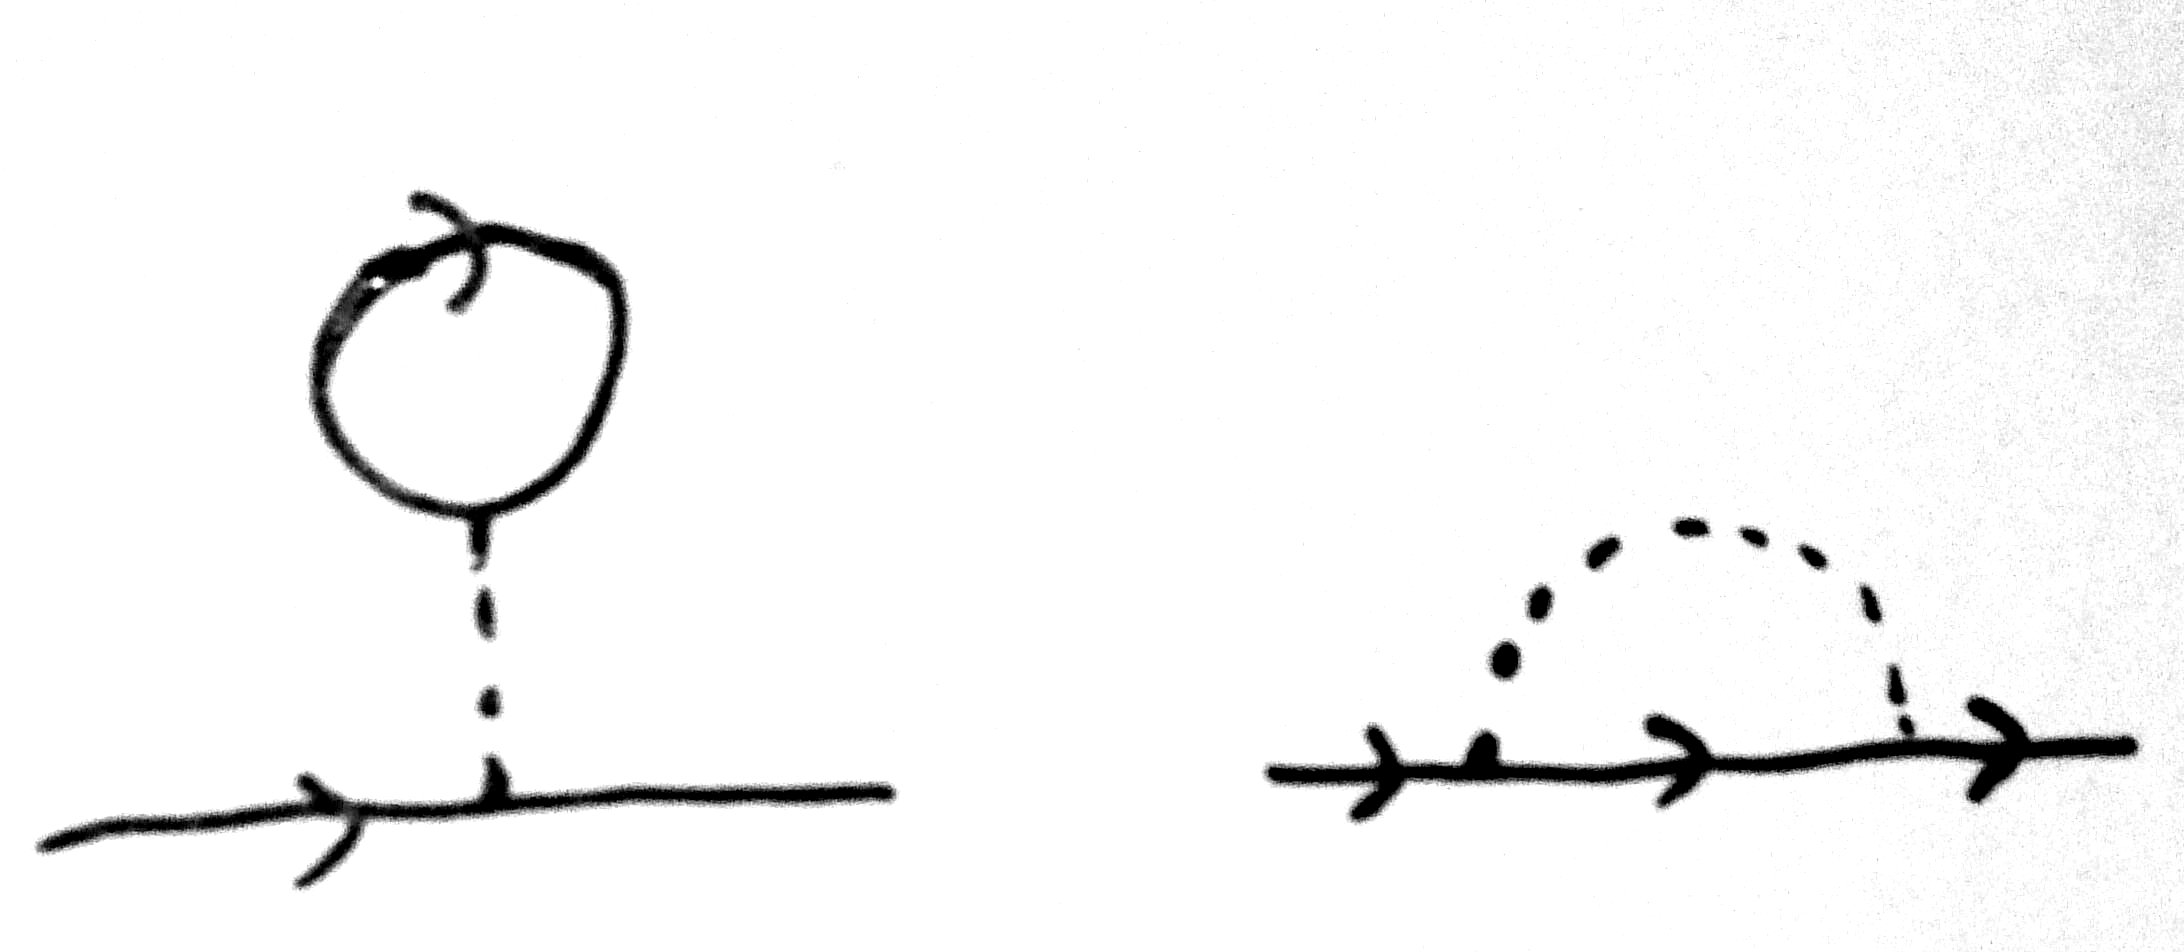
\includegraphics[width=10cm]{Zero/1stFDiagram.jpg}
\caption{一阶连接图}
%\label{default}
\end{center}
\end{figure}

\item

引入连接图和非连接图概念后,格林函数可表示为:

\begin{equation}
iG = \frac{\left\langle \Phi_0 \right| T ( \psi \psi^\dagger S ) \left| \Phi_0  \right\rangle_c \times \left\langle \Phi_0 \right|  S  \left| \Phi_0 \right\rangle_{nc}}{ \left\langle \Phi_0 \right|  S  \left| \Phi_0 \right\rangle_{nc}} = \left\langle \Phi_0 \right| T ( \psi \psi^\dagger S ) \left| \Phi_0 \right\rangle_c
\end{equation}

即格林函数可表示为所有拓扑不等价的连接图形之和!

\begin{figure}[htbp]
\begin{center}
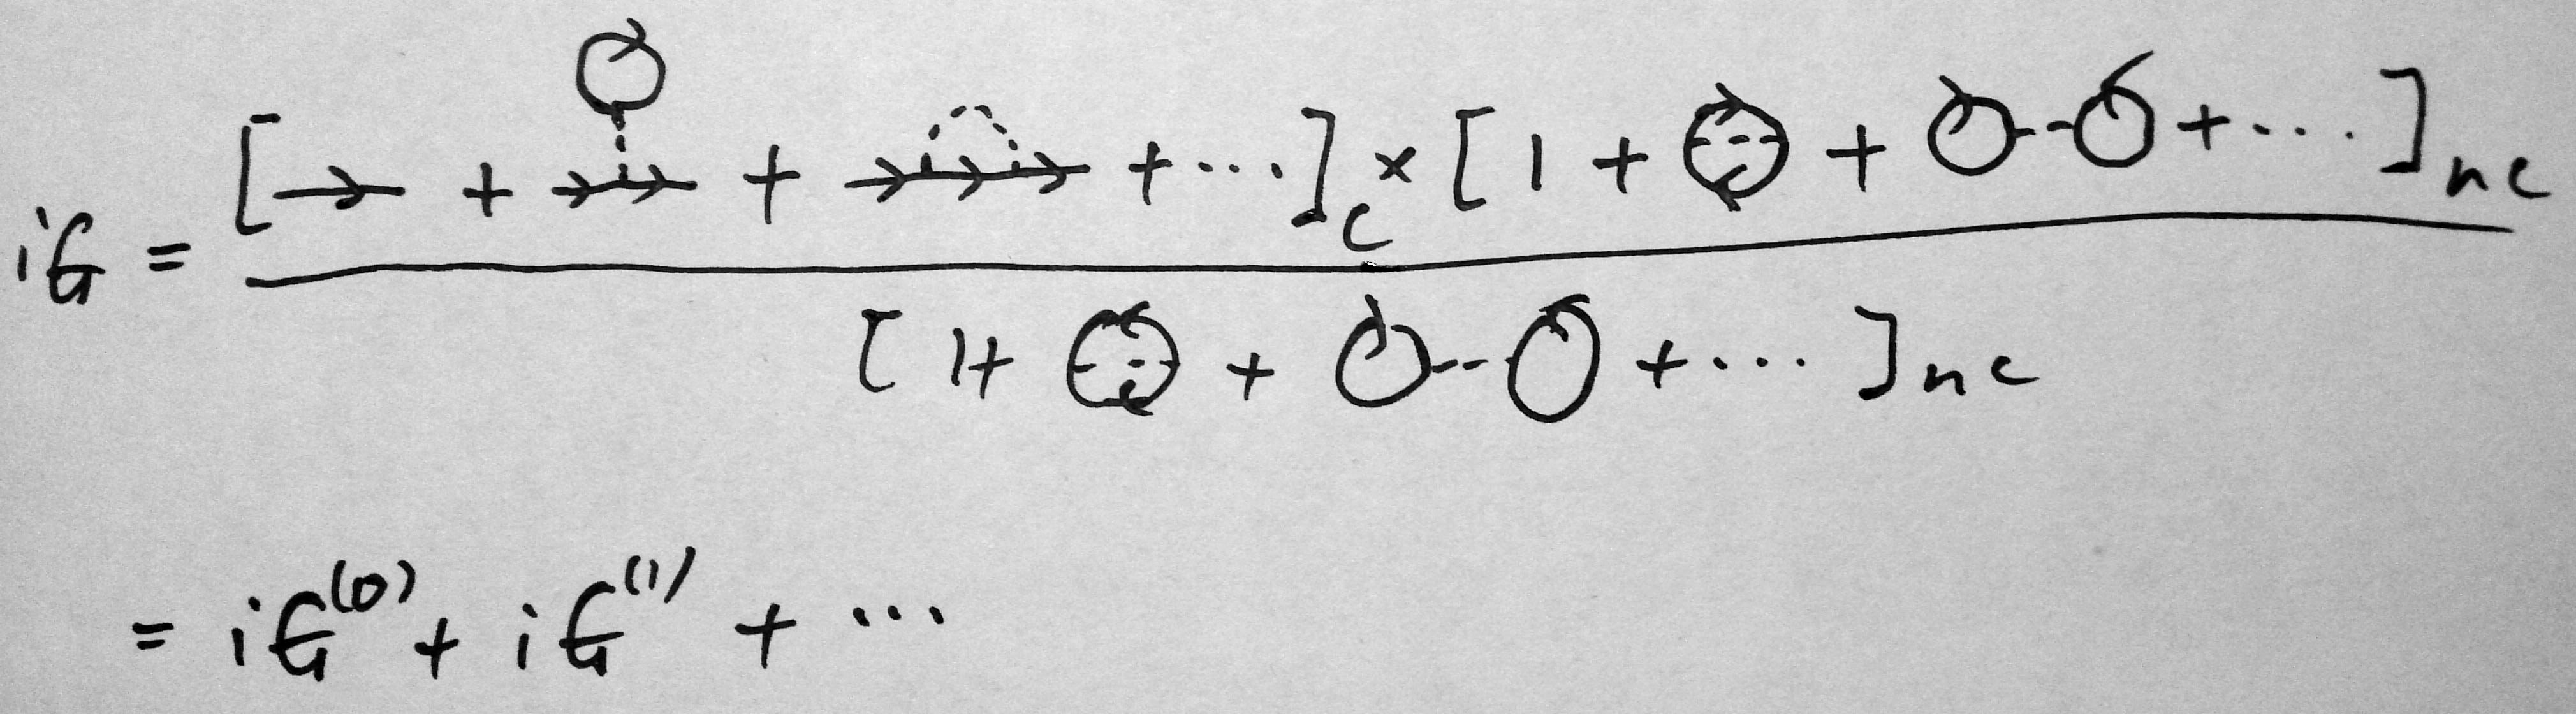
\includegraphics[width=11cm]{Zero/FDconnected.jpg}
\caption{非连接图形的部分正好被消掉了。}
%\label{default}
\end{center}
\end{figure}

\item

对从一点出发又回到这一点的单粒子线,或连接在相同相互作用线上的粒子线,时间宗量相同,此时我们必须规定:T乘积内$\psi^\dagger$的时间要比$\psi$的大一个无限小量$\eta$。

\begin{equation}
i G^0 (x , x) = \left\langle \Phi_0 \right|  T (\psi(x,t) \psi^\dagger (x,t+\eta) ) \left| \Phi_0 \right\rangle = iG^0 (-\eta)
\end{equation}

同时,

\begin{equation}
i G^0 (x , x) = - \left\langle \Phi_0 \right| \psi^\dagger  \psi   \left| \Phi_0 \right\rangle = - n^0 (x)
\end{equation}

\item 

一个闭合粒子线对应一个“-”,相当于有一个传播子是从未来传回来的。在$G^{(n)}$中如果有$F$个闭合粒子线,则有因子$(-1)^F$。

\end{enumerate}


\subsection{动量空间的图形规则}


\begin{enumerate}

\item 

\begin{eqnarray*}
G(x,y) & = & (2 \pi)^{-4} \int d^4 k  e^{i k \cdot (x-y)} G(k) \\
U(x, x') & = & (2 \pi)^{-4} \int d^4 k e^{i k \cdot (x-x')} U(k) \\
\end{eqnarray*}

这里$d^4 k \to d^3 k d \omega$, $k \cdot x \to k \cdot x - \omega t $

\item

对每个内定点,动量、能量守恒:

\begin{equation}
\delta^{(4)} (q - q' + q'') = (2 \pi)^{-4} \int d^4 x e^{i (q- q' + q'') \cdot x}
\end{equation}

\item

对$G(k,\omega)$的第n级贡献$G^{(n)} (k, \omega)$,

首先画出n根相互作用线,和$2n + 1$根有向粒子线的所有拓扑不等价的连接图形。

\item

对每个内定点要求动量-能量守恒,总共有$2n$个守恒条件。

\item 

对内线的自旋指标求和。

对$n$个独立的内部四维动量(哑元)积分。

(总共有$3n + 1$个粒子线或相互作用线,去掉$2n$个守恒条件,再去掉1个外线,还剩$n$个独立的内线。)

\item

每一项附加因子

\begin{equation*}
i^n (2 \pi)^{-4n} (-1)^F
\end{equation*}

这里$F$是闭合费米子线的个数。

\item

对每个形成闭合环的单粒子线,或与同一根相互作用线相连的单粒子线。

对$G(- \eta)$做傅里叶变换,为:$e^{i \omega \eta} G(k, \omega)$

\end{enumerate}

作为练习,我们可计算动量空间中的一阶图形。

\begin{eqnarray*}
G^{(1)} & = & G^{(1)}_a + G^{(1)}_b \\
G^{(1)}_a & = & i G^0 (k) (2 \pi)^{-4} \int d^4 p V(k-p) G^0 (p) G^0 (k)  \\
G^{(1)}_b & = & i (-1) G^0 (k) (2 \pi)^{-4} \int d^4 p G^0 (p) V(0) G^0 (k)
\end{eqnarray*}

这里:$G^0 (p) \to e^{i \omega \eta}  G(p, \omega)  $


